
 \chapter{Preprocessing}
 \label{chpt-preprocessing}
 \nomenclature[1]{INN}{International Nonproprietary Name} 
 \nomenclature[1]{BAN}{British Approved Name}
 \nomenclature[1]{USAN}{United States Adopted Name}
 
 
 
 \section{Introduction}
 
In order to improve classifier performance we sought to develop preprocessing methodologies that would improve the quality of text which would be developed into word embeddings. The primary goals of this work was to provide feature reduction and error correction. 

The issue to be addressed in preprocessing was the noisy, high dimensional recording of two different types of potentially useful terms within the FTN: namely that of medications and contractions. We detail in this chapter the issues found in relation to these two aspects of the FTN, the approaches we used to address these problems, and the ultimate performance and limitations of the methodologies that were developed.



The hypothesis was that providing more abstract versions of terms in text would ultimately improve classification capacity. Alternatively, some high value terms could be hidden within acronymised forms. 

\hl{
The methodologies discussed in this chapter use the entire volume of free-text data contained within the corpus, as described in Section} \ref{section:free-text-description}, for all training and text transformation operations. The contents of this chapter were in part published in IADIS 2017 `Abbreviation and Acronym Identification and Expansion Within Medical Health Records' \cite{wallace2017abbreviation} and `Retrieval and Clustering of Medicines Within Healthcare Data Records' \cite{wallace2016retrieval} in BDAW 2016 which sought to identify means of identifying and correcting both contractions and medications in the corpus, respectively.

\section{Medication Reconciliation}
\label{section:medication-reconciliation}

As mentioned in Chapter \ref{chpt:background}, the free-text medication data in EHR\index{Electronic Health Record} is predominantly unsanitised, and its unstructured nature makes it inaccessible to other computer applications that rely on coded data in healthcare settings (e.g, electronic medication reconciliation systems), as well as clinical research that uses structured medication data, such as EHR\index{Electronic Health Record}-based \cite{kushima2012text}. Despite providing a means of reducing paper-based inaccuracy, Electronic Medical Record Management systems are still subject to human error \cite{koppel2009emr}.

Medication reconciliation is a formal process for creating a more complete and accurate list of a patient's medications for the purpose of supporting correct medication orders. Given the increasing use of EHRs\index{Electronic Health Record}, automated medication reconciliation methods have received great attention \cite{grossman2014hospital}. One particular challenge involves the heterogeneity of clinical data, which consists of both coded and narrative medical data \cite{michaelsen2015medication}.

Despite the inherent value that these terms bear, free-text medical information may contain large volumes of pharmaceuticals recorded inconsistently, both stylistically and structurally. The pharmaceuticals themselves may be incorrectly recorded, and no list of pharmaceuticals likely to recorded in a corpus may exist. The purpose of this part of the research is to develop a system that can extract drug names from this unstructured data in order that this information be available for analytical purposes, both on a population and individual basis. In this way it may be possible to provide useful and interesting inferences over large volumes of data.




This section will examine the ways in which pharmaceutical discovery can be achieved, before looking at the ways in which this thesis' methodology was implemented. The proposed solution will build upon extant research, as described in Section \ref{section-rr-medication-identification}. The methodology will focus on environmental analysis of the text and, as such, a subsection will explore the manner in which this was conducted. Finally, the results of the information retrieval and success of the clustering of such terms is analysed.   




\subsection{Problem Definition}

 While drug names tend to follow certain morphological conventions, these not only pose a problem by their sheer volume, but even presupposing that pharmaceuticals are recorded using full international non-proprietary name \\ (INN) \cite{dunne2013review}, stems used to denote drugs are syntactically so sparse as to preclude any sort of acceptable precision. Naturally, such affixes and suffixes are unlikely to relate to proprietary names under which these products are marketed, which may be the manner in which drug products are represented within the text. As such, the analysis of words, in isolation, to discover medications within the text can be discounted. 
 

Instead, an analysis of the structure of medical notes to detail the types of syntax which are likely to indicate the presence of medications will be conducted. Although the heterogeneity of free-text notes precludes certain NLP\index{Natural Language Processing} measures, developing simple syntactic patterns has the potential to accurately return medication names within such notes.

It is a primary ambition of this part of the research to deliver a system that can not only identify the proprietary, trade and generic names of pharmaceuticals, but provide also the means for incorrectly transcribed pharmaceuticals occurring within free-text notes to be automatically corrected with a high degree of precision. 


This chapter aims to discover a broad spectrum of medications, but will consider all other lexemes to be incorrect. For instance, the term ``antibiotic" would be considered to be a valid medication name (despite its generic nature) while a word like ``emulsion", which denotes a delivery method for medications, would be considered incorrect. All lexemes which denote medications, but are incorrectly spelled (for instance \textit{prendnesol} instead of \textit{prednesol}) will be considered erroneous.  

\subsection{Proposed Solution}
\label{section:prescription-solution}

Using a predefined list of drug names (namely using RxNorm\index{RxNorm}), co-occurring terms found within the text will be collected, excluding stop words.  The highest frequencies of co-occurring lexemes will next be compared against one another in order to develop well defined environments within which medications are likely to be present. 

Once structures which telegraph the presence of medication details have been defined, suitable structures will be used to collect lexemes which may represent medications.  The data collected will exclude common English words and lexemes less than three characters in length (as the latter are too short to relate to pharmaceutical names). The accuracy of the pattern used to discover candidate medications names will underpin the precision of the overall program, as both unrelated medical words, and misspelled words that do not relate to medications are otherwise likely to be returned by this process.

\hl{Data relating to common English words was derived from a truncated version of SCOWL}\index{Spell Checker Oriented Word Lists}, of size 35 (the recommended `small' size of the SCOWL repository, where `size' is synonymous for how common the specific lexemes are)\cite{atkinson2004spell}. This dataset, reportedly around 7.6\% of the total volume of SCOWL lexemes, totalled some 50,000 words. The rationale for using this particular subset of the SCOWL dataset was its purpose in excluding common, non pharmaceutical lexemes in the following tasks. A much larger version of SCOWL could potentially run the risk of excluding some true positive pharmaceutical candidates.

By searching all other text for occurrence of the collected words, a dataset of pharmaceuticals and their frequency within the EHR\index{Electronic Health Record} can be established. The collection of drug and product names above is guaranteed to return many errors, both typographical and cognitive in nature, where users have entered the names of products they are describing incorrectly. Common English words which have been misspelled, and domain-specific terms alike may also hypothetically be collected in this process. Furthermore, terms that are four characters in length are overwhelmingly likely to represent domain-specific acronyms, or product name contractions. However, by analysing both the frequency of occurrence and morphological similarity of the terms collected, it is intended that the program will automatically correct these errors.
 




%\begin{figure}[!t]
%\centering
%\includegraphics[width=2.5in]{workflow.png}
%% where an .eps filename suffix will be assumed under latex, 
%% and a .pdf suffix will be assumed for pdflatex; or what has been declared
% \DeclareGraphicsExtensions.
%\caption{Overall program structure.}
%\label{workflow}
%\end{figure}



\subsection{Methodology} 
 \label{section:pharmaceutical-retrieval-methodology}
 
%The data provided, which had previously been anonymised, was cleaned of duplicate entries and tokenised. The preprocessed text was analysed for sentence structures which would indicate the presence of prescription details. Terms in proximity to numerical tokens succeeded by prescription related lexemes were collected as candidate names.

By taking the list of drugs presented within RxNorm\index{RxNorm} the frequencies of all co-occurring words were recorded. Co-occurring words could appear immediately before or after the name being searched, provided that it was not interceded by punctuation (newlines, periods, etc.). Stopwords were excluded from this process using the twenty five semantically non-selective words which are common in Reuters-RCV1\cite{sanderson2010christopher} \footnote{This list can be viewed in Table \ref{table:app-stopwords} in the Appendices.}.
 A very small stopword list was demanded for this task, in order to avoid accidentally filtering important neighbouring terms during analysis, hence the choice of this particular list. 

Having collected the frequencies of co-occurring words, work was begun on creating a co-occurrence network in order to identify structures within the text that pharmaceuticals are likely to be found. Analysis of the interconnection between the top forty terms was conducted. Interconnection was determined by simultaneous presence of terms on the same line of text within the corpus of free-text notes. 

While mutual information may theoretically have produced more accurate results in this regard \cite{nakagawa2003automatic}, this process was merely exploratory in nature, whereby the identification of medication contexts was a means to an end to discover medication candidates. These candidates in turn would be leveraged to identify further candidates. 

In order to eliminate the long tail of infrequent terms, the co-occurrence network eliminated nodes that failed to have any edge with a weight within the top half of occurrences. This approach was appropriate given the immediate demand to identify the most typical environment within which medication terms might occur. Finally, modularity of the network was conducted, separating the network into three distinct classes using Blondel et al.'s clustering algorithm \cite{blondel2008fast}, as can be seen below in Figure \ref{network-drugs}. Despite mutually exclusive clusters, very strong connections between terms in one cluster and terms in another cluster may exist  (e.g. between `pain' and `po').

The orange coloured community represents paediatric related contexts. Nurse triage staff answering paediatric related cases may advise the use of non-prescription based medicines in many cases in order to ease the symptoms relating to the child's complaint. This context consequently tends towards a relatively limited number of medications which occur in high frequency. This can be observed in the presence of a pharmaceutical name which has actually appeared within this cluster (namely `calpol').

The second community identified (green) is a more generalised context relating principally to initial contact between a patient and phone operator where non-specific details may be related. While the lexemes in this group have a relatively strong correlation with medications, and a particularly high correlation with one another, the high variance of types of information related in the proximity of these terms augurs poorly for the precision of medicine based information retrieval. 

Prescription details (purple) closely mirror their real-world handwritten equivalents, both in terms of register and structure. As such, the invocatio of the praescriptio typically contains weights and measures \cite{hadavsova2009practicals}. This generates a consistent pattern of drug or product names, succeeded by measurements (that may change temporally), which may be followed by some temporal value. These prescription details may be singular or composite.

When looking for non-lexical co-relation with the different classes, prescription based words had a particularly strong relationship with numerical elements. Lexemes belonging to the prescription class had a total of 100,669 numerical co-occurrences compared with 3,654 for general and 12,954 for paediatric contexts. 

Taking account of the semantic ordering of prescription related terms, certain patterns became apparent, with particular terms tending towards different relative positions. When grouping the terms by meaning (relating to quantifiable and temporal specifications), the most common semantic structure was for numerical tokens to be followed by quantification and temporal tokens, in that order (with some 25,618 occurrences). The second most common structure was for numerical tokens to be followed simply by quantification tokens (with some 16,617 occurrences).  

Using this as a means by which to proceed, the preprocessed text of the corpus was analysed for sentence structures which would indicate the presence of prescription details. Terms in proximity to numerical tokens, succeeded by prescription related lexemes in the order hitherto observed, were collected as candidate names. Terms which were within SCOWL \index{Spell Checker Oriented Word Lists} were excluded, while those less than three characters in length were discarded in favour of the nearest suitable lexeme. 



    \begin{figure}[!ht]
      \centering

      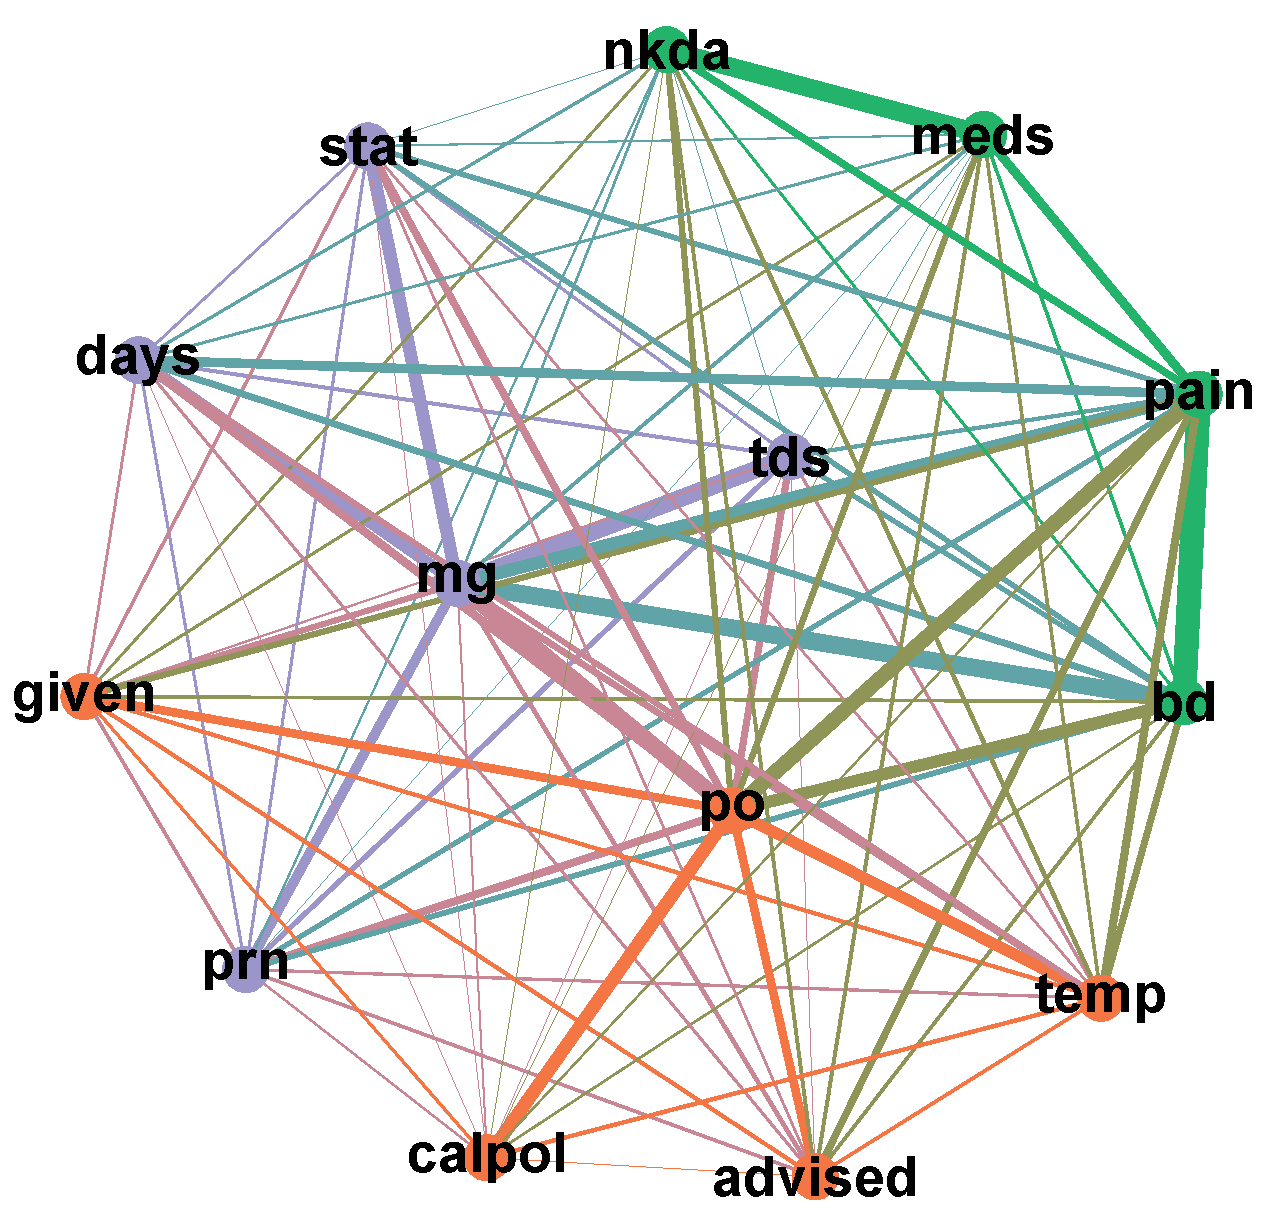
\includegraphics[scale=0.5]{network-drugs.pdf}
      
      \caption{Undirected graph of context relations.}
      \label{network-drugs}
   \end{figure}


%In order to determine the accuracy of the program an exhaustive search was conducted through various media to ascertain whether each of the recorded candidate names was a correctly written pharmaceutical. 

Following the collection process, a frequency was taken of all collected candidate names within the entire training corpus. This was done so that the recorded frequency would reflect the general preponderance of candidate names within the text, not limited solely to the context of prescriptions.

Of the terms collected, names that were were exactly four characters in length overwhelmingly represented false positives or abbreviated forms of drug names. Contracted forms of drug names typically have very large edit distances from their full length versions, so a specific process of contraction inflation was developed. This process analysed the longer candidate medication names for a potential match, based both upon length and morphological similarity. In the event of a conflict, the full-length candidate name with a greater frequency was chosen. Any term which ultimately found no suitable match was removed from the list of candidate names.

Finally, the edit distance between candidate pharmaceuticals was tested using an implementation of the Levenshtein distance string metric \cite{schulz2002fast} (see \hl{Figure} \ref{euclid}). The hypothesis was developed that supposed that the edit distances would be predominantly short between incorrect pharmaceutical entries and their correct versions, and that, as a general principle, incorrect edits would necessitate longer edit distances \cite{hodge2003comparison}.  This was implemented using varying distance criteria, and the results recorded \hl{(see Table} \ref{table:lev-distance1}).

%INSERT MATHEMATICAL FORMULA INSTEAD OF PSEUDOCODE HERE


\begin{figure}
\begin{algorithmic}[1]
\Procedure{editDistance}{$s1,s2$}
\State $a[i,k] =0$
\For{$i = 1 \to  |s1|$}
\State {$a[i,0] = i$}
\EndFor
\For{$k = 1 \to  |s2|$}
\State {$a[0,k] = k$}
\EndFor
\For{$i = 1 \to  |s1|$}
    \For{$k = 1 \to  |s2|$}
    \State {$a[i,k] = \min\{a[i-1,k-1]+$}
    \If{$(s1[i]=s2[k])$}
        \State{$0$} 
    \Else 
    \State{$1$} 
    \EndIf
    \State {$a[i-1,k]+1, a[i,k-1]+1$}
    \EndFor
\EndFor

\State \textbf{return} $a[|s1|,|s2|]$
\EndProcedure
\end{algorithmic}
\caption{Levenshtein distance.}\label{euclid}
\end{figure}


%\subsection{Results}

Candidate medications were collected from the dataset through the identification of prescription details. This resulted in 3,778 candidate pharmaceutical names being obtained. When searched for through the entire corpus, it was found that these candidate names related to some 460,232 occurrences within the entire text.  

However, of these candidate names, only 896 terms were correct (being both actual pharmaceuticals, and correctly spelled). Of the 2,893 incorrect candidate names, the vast majority represented incorrectly spelled drug names, with only 98 falling into other categories (predominantly relating to abbreviated forms of drugs and routes of administration). Incorrect terms accounted for roughly half the population of candidate instances within the corpus (152,500 versus 155,295).


\subsection{Abbreviation Inflation}

A very simple means of dealing with abbreviated pharmaceutical names was devised that would attempt to match short candidate names that were collected during the information retrieval task detailed in Section \ref{section:pharmaceutical-retrieval-methodology}. This program would try to find another candidate name, of which the proposed abbreviated pharmaceutical was a substring, and delete the proposed abbreviation if no match was made. This program was run on the 86 candidate names which were 4 characters in length. This resulted in one false-negative being deleted (a drug with some 569 occurrences in the corpus), and two false-positives, where drugs were wrongly inflated to larger forms (accounting for 17 occurrences together). 

Twenty-eight true-positives were identified and correctly inflated (totalling some 2990 occurrences), although two of these candidates were inflated to words which were themselves incorrect candidates: namely nebulizer (61) and suppository (52), both of which are routes of administration rather than pharmaceuticals.

An additional fifteen abbreviations (totalling 89 occurrences) were incorrectly identified as being pharmaceutical abbreviations and were added to the count of extant drugs.

Forty-two abbreviations were deleted, thirty eight of which were correctly identified as being unrelated to any larger form, such as `meds' and `stat'. These thirty-eight abbreviations which were deleted accounted for a substantial population, relating to 108531 occurrences within the corpus. The four abbreviations which were incorrectly deleted were somewhat aberrant in that their abbreviated forms did not match their full length counterparts (such as penv and phenoxymethylpenicillin). These false-negatives related to sixty-five occurrences in the corpus.

The abbreviation-inflation described above had a marginal effect on the average length of candidate names, whereby an increase was observed of the plain average of names, where candidate names are treated as a set, from 8.86 to 8.97, and an increase of the weighted average, where candidate names are treated as a multiset, from 7.046 to 8.03. However, this process had a substantial impact on the standard deviation of incorrect candidate names, decreasing from 1439.264 prior to inflation, to 132.827 afterwards).

\subsection{Edit distance}
\label{section:medication-collection}

Once the abbreviation inflation had been concluded, the edit distances of all candidate names were tested against one another using a varying distance parameter (see Table \ref{table:lev-distance1}). The aim of this comparison was to not only remove incorrect candidate names, but to also add the count of incorrect candidates to their corrected versions, where applicable. 

It was expected that a higher edit distance would result in higher true positive changes, but with a corresponding rise in false positives. As it was unclear, \textit{a priori}, what kind of ratio this would have, the results from edit distances between one and four (inclusive) were recorded (Table \ref{table:lev-distance1}). 

Corrections from one true (\textbf{t}) form to another true form is considered fallacious, as this is more likely to result in a pharmaceutical being corrected to an unrelated pharmaceutical. Yet, even if the correction is to a related product, this represents a form of generalisation not specifically sought within the scope of this research. Alteration of correct pharmaceutical names to incorrect versions are in particular to be avoided, as this not only removes a correctly identified medication from our list, but gives undue weight to incorrect entries. Corrections from one incorrect entry to another are predominantly beneficial, as not only is an incorrect entry removed from the list in this process, but it is possible that the form to which it has been corrected may act as an incremental step towards the appropriate spelling of the pharmaceutical. 





\begin{table} [ht]
%% increase table row spacing, adjust to taste
\renewcommand{\arraystretch}{1.6}
\setlength{\tabcolsep}{0.7em}
% if using array.sty, it might be a good idea to tweak the value of
% \extrarowheight as needed to properly center the text within the cells
\caption{First iteration of edit distance.}
\label{table:lev-distance1}
\centering
\begin{tabular}{@{}c|c|c|c@{}}
\toprule
\textit{distance}   & \textbf{f$\rightarrow$t} & \textbf{t$\rightarrow$ t} & \textbf{t$\rightarrow$ f} \\ \midrule
\textit{\textbf{1}} & 1587                     & 47                        & 19                        \\ \midrule
\textit{\textbf{2}} & 2572                     & 137                       & 36                        \\ \midrule
\textit{\textbf{3}} & 2483                     & 394                       & 56                        \\ \midrule
\textit{\textbf{4}} & 2757                     & 821                       & 45                        \\ \bottomrule
\end{tabular}
\end{table}

\begin{figure*}[ht]
\centering
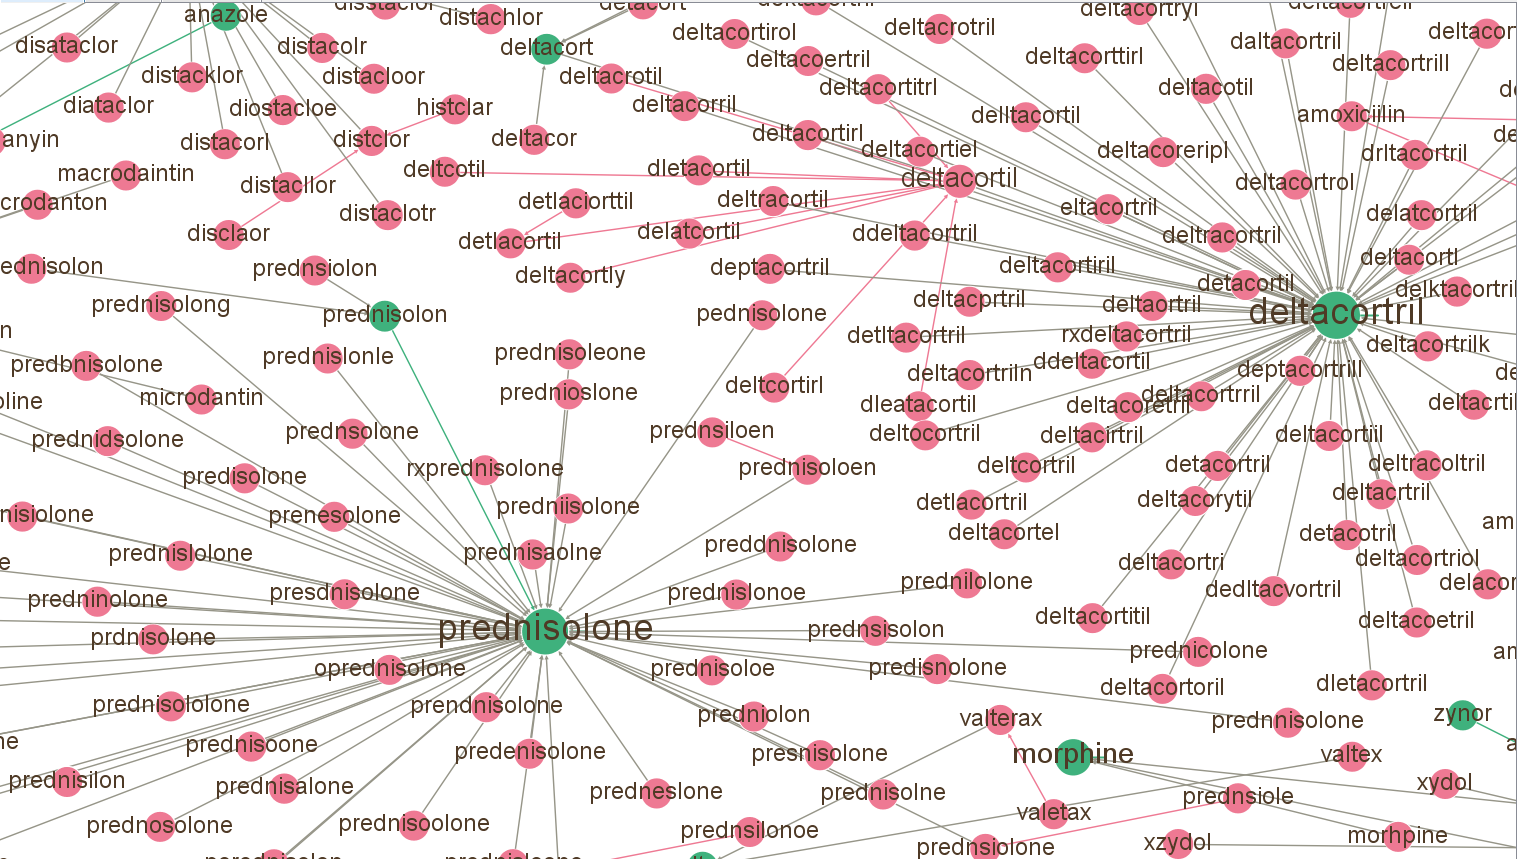
\includegraphics[width=\textwidth]{replace_drugs.PNG}
% where an .eps filename suffix will be assumed under latex, 
% and a .pdf suffix will be assumed for pdflatex; or what has been declared
\DeclareGraphicsExtensions.
\caption{Network simulation of correction decisions at a distance of two.}
\label{network}
\end{figure*}

A network representation of this process can be observed in Figure \ref{network}, where the edit distance is set to two. Green nodes represent correct candidate names, while red nodes represent incorrect ones. Node sizes represent the number of occurrences within the text.

As can be seen in Table \ref{table:lev-distance1}, edit distances of three and four had had significantly inferior performance (relative to the number of errors generated) and subsequent testing was consequently conducted using edit distances of one and two. These edit distances, visible in Table \ref{table:lev-distance2}  were executed on the previous results relating to edit distances of one or two, in order to explore whether increased accuracy might be generated by this process.






\begin{table}
\renewcommand{\arraystretch}{1.6}
\setlength{\tabcolsep}{0.7em}
% if using array.sty, it might be a good idea to tweak the value of
% \extrarowheight as needed to properly center the text within the cells
\caption{Second iteration of edit distance.}
\label{table:lev-distance2}
\centering
\begin{tabular}{@{}ccccc@{}}
\toprule
\textit{initial step}                            & \textit{second step}            & \textbf{f$\rightarrow$t} & \textbf{t$\rightarrow$ t} & \textbf{t$\rightarrow$ f} \\ \midrule
\multicolumn{1}{c|}{\multirow{2}{*}{\textit{1}}} & \multicolumn{1}{c|}{\textit{1}} & \multicolumn{1}{c|}{203} & \multicolumn{1}{c|}{9}    & 1                         \\
\multicolumn{1}{c|}{}                            & \multicolumn{1}{c|}{\textit{2}} & \multicolumn{1}{c|}{568} & \multicolumn{1}{c|}{95}   & 11                        \\ \midrule
\multicolumn{1}{c|}{\multirow{2}{*}{\textit{2}}} & \multicolumn{1}{c|}{\textit{1}} & \multicolumn{1}{c|}{84}  & \multicolumn{1}{c|}{11}   & 3                         \\
\multicolumn{1}{c|}{}                            & \multicolumn{1}{c|}{\textit{2}} & \multicolumn{1}{c|}{127} & \multicolumn{1}{c|}{45}   & 35                        \\ \bottomrule
\end{tabular}
\end{table}



The most successful route of edit distance correction involved an iterative process of correcting to a distance of two, and then correcting again to a distance of two on these results. 

\begin{table}
\renewcommand{\arraystretch}{1.6}
\setlength{\tabcolsep}{0.7em}
% if using array.sty, it might be a good idea to tweak the value of
% \extrarowheight as needed to properly center the text within the cells
\caption{Pharmaceutical test results.}
\label{table:pharmaceutical-testing}
\centering
\begin{tabular}{@{}lccc@{}}
\toprule
                  &                           & correct edit & incorrect  edit \\ \cmidrule(l){3-4} 
initial incorrect & \multicolumn{1}{l|}{33.1} & 84.78        & 2.17            \\
initial correct   & \multicolumn{1}{l|}{76.9} & N/A          & 2.15            \\ \bottomrule
\end{tabular}
\end{table}

This process left 728 correct pharmaceutical names out of a total of 977 candidate names. However, a substantial number of these medications appeared only once within the entire corpus. These 200 single instance candidate names, which were predominantly incorrect (146 false to 34 true) could be discounted as outliers and removed. This left 685 true to 95 false candidate names: representing an overall accuracy of 88.15\%. When taking volume of occurrence into account, the retained candidate names represent an accuracy of 93.6\%

This final result represents an over 57\% rise in the precision of candidate names, from an accuracy of only 30.97\% of \hl{candidate pharmaceuticals collected during the initial information retrieval detailed in Section} \ref{section:pharmaceutical-retrieval-methodology}. Of the initial 896 correct candidate names identified, 76.45\% were retained. However, if we discount outliers, this retention rises to 82.63\%. Looking at the numbers that the surviving candidates relate to, we see 359,207 occurrences, of which \hl{334,599} relate to correct pharmaceutical names. However of this number  9870 instances relate to one correct pharmaceutical being wrongly corrected to another.

Taking a random sample of 200 records that were hand annotated by a domain expert for testing purposes (Table \ref{table:pharmaceutical-testing}), the program's training data achieved an 82.56\% recall. Of the pharmaceuticals correctly identified, 33.1\% were incorrectly spelled or written, of which 84.78\% were successfully corrected by the program, 15.21\% were unchanged and 2.17\% were incorrectly changed. Of the 76.9\% of the pharmaceuticals identified which had been correctly spelled, a further 2.15\%  were erroneously changed.

\subsection{Discussion}

The most apparent finding from the results is that automatic correction of pharmaceuticals necessitates very large volumes of data for accurate results. The greater the volume of data presented, the more likely that drugs will appear in the context of prescriptions and be caught by the information retrieval methods designed specifically to parse these structures. Moreover, the greater the volume of data collected, the easier it is to identify false positives and incorrectly recorded pharmaceuticals. 

While the contextual analysis performed relatively well in excluding unrelated domain-specific terminology from results, 11 of the 777 final candidate pharmaceutical names were such terms (for instance `paediatric' and `suppos'). A possible solution to this would be to clean final results with a more extensive dictionary than that used in the course of this chapter. It would not be advisable to use this larger dictionary to filter pharmaceuticals at the beginning of the collection process, as both abbreviations and variant spellings were clustered on these terms in the course of the program. However, the fact that 7 of these terms tend to appear in quite close proximity to prescription details may indicate a means of exclusion through contextual analysis. The 18 incorrect candidate names which represent misspelled English words (such as `injeciton', `depressent', and `strenght') may potentially be targeted in a similar manner.

The program is fundamentally dependent on users predominantly writing correct versions of pharmaceuticals, and cannot account for particularly prevalent cognitive mistakes \cite{sessions2006effects}. For instance, a majority of users believed that amoxicillin was spelled amoxycillin in the corpus. This had the effect of inadvertently causing the correct version of the drug name to be clustered on the incorrect version \footnote{While not very relevant to our purposes of using this preprocessed data for classification of frequent users, this taxonomic error was automatically fixed in Section \ref{section:dbpedia}}. 

%Finally, in a handful of cases contracted forms of pharmaceuticals were longer than was originally expected, e.g. `fluclox' (for `flucloxacillin'). A relatively trivial solution is to automatically inflate candidate names which are affixes of longer alternatives. 

While a conservative ceiling on edit distances will reduce the identification of false negatives \cite{jupin2012understanding}, there is no means to eliminate all possible false negatives without recourse to some sort of ontology.

Using a predefined list of pharmaceuticals to develop a topographical understanding of context has proven a suitable means to discover pharmaceutical environments. However, while context has clear application in identification of medications within free-text notes, a more syntactically sensitive approach may yet yield stronger results in terms of both recall and precision. Nevertheless, the process exhibited in this chapter has strong performance in both these categories. In particular, the capacity of the method described to discover hitherto unknown pharmaceuticals has obvious application. Non-trivial exclusion of false-positives is an ongoing concern. Furthermore, the method described does not itself provide any information about the relationships of true-positive pharmaceuticals to one another, and many different products may be recorded that have similar, or even identical functions.     



\subsection{\hl{Feature Reduction}}
\label{section:dbpedia}


Reduction of synonymous features is a useful step in the preprocessing of data prior to its use in machine learning and data mining applications. One of the most important features in clinical free text is the prevalence of pharmaceutical names. These names vary from local brand names to internationally recognised drug names. Local brand names, while understandable to people living in the area in which the data is being recorded, have the potential to obfuscate the general type of medication that is being discussed. As such, a means to abstract pharmaceuticals to a higher level, from an ontological point of view, would likely reduce ambiguity within text.

To this end the viability of many official pharmaceutical repositories, such as RxNorm \index{RxNorm} \cite{nelson2011normalized}, were examined. This was done with the hope of being able to resolve these ambiguous names. However, many of these repositories tended to feature relatively limited capabilities in mapping of proprietary to non-proprietary names, and a conspicuous absence of the types of local trade names which are specific to the environment in which our corpus was created. Consequently, these repositories provided little applicability to our needs. Instead, the ontological representation of Wikipedia, namely in the form of DBpedia\index{DBpedia} \cite{lehmann2015DBpedia}, provided a viable platform for this type of feature reduction.


One of Wikipedia's core tenets is that different pages should not exist on the same topic. Specifically, it has a policy against content forking where redundant information may be produced. Duplicate content may be deleted, or merged with preexisting articles. In order to aid both navigability and search optimisation, redirects exist to point synonymous terms (or variant spellings) to a particular article. Specifically in relation to drugs, Wikipedia's policies state that article titles should be their International Nonproprietary Name (INN) \cite{kopp1995international}, while other identifiers (such as The British Approved Name (BAN) \cite{british2002british} or United States Adopted Name (USAN)\cite{boring1997development} variants)  may also be mentioned in the lead section of articles. Consequently, proprietary and common names of pharmaceuticals typically exist solely as redirects to articles listed under the product's INN.

While DBpedia\index{DBpedia} is a structured hierarchical form of Wikipedia, it maintains metadata relating to the type of redirects described above (in accordance with the Linked Data principle \cite{bizer2011linked}) . Pharmaceutical names have previously been collected from our corpus and cleaned using information retrieval methods and clustering in Section \ref{section:medication-collection}. Using this list of pharmaceuticals against the DBpedia\index{DBpedia} API, XML featuring the labels relating to the respective medication articles hosted on Wikipedia could be derived. \hl{Using this methodology the number of distinct pharmaceuticals could be significantly reduced within the corpus through substitution with the parsed XML labels.} 


\begin{figure}[h]
   \centering
   \begin{tabular}{@{}c@{\hspace{.5cm}}c@{}}
 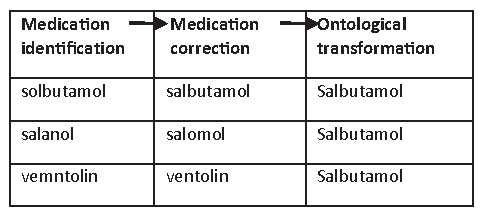
\includegraphics[page=1,width=.80\textwidth]{druggy3.pdf} & 
   \end{tabular}
  \caption{Sample identification, lexical correction, and transformation using DBpedia\index{DBpedia}, in relation to medications within the unstructured textual notes.}
 \label{druggy}
\end{figure}

An example of this process can be seen in Figure \ref{druggy}.  The results of this process was the reduction of pharmaceuticals from 777 distinct classes (excluding single entry medications) in the entire corpus to only 309 (though 8 pharmaceuticals were disambiguated to two separate classes)\footnote{While disambiguation was not behaviour particular sought after in this process, it was not, strictly speaking, in error.}. Moreover, only 189 pharmaceuticals remained entirely unchanged,  with the remaining 588 being resolved to a more generic variant.




%SHOW THE PROCESS OF CHANGING A SINGLE DRUG NAME TO GENERIC FORM




A perennial issue in relation to contractions is the ambiguity inherent in potential reading, when canonical definitions are not provided in the text. Unlike scientific journals, medical free-texts typically do not provide glossaries or in-line explanations of contractions, and even where an organisation may provide guidelines concerning the use of acronyms and abbreviations; these may not necessarily be followed by individual users\footnote{ Caredoc\index{Caredoc}, as previously mentioned, does not possess any guidelines on the use of abbreviations and acronyms by its staff.}. Moreover, synonymous terms may be recorded as morphologically unique contractions. 

Semantic details proved poor at identifying contractions. However, it was discovered that contractions had a number of distinguishing syntactic characteristics within free-text. Although a number of these identifiers may exist simultaneously, at times none of these characteristics may be present as writing styles vary greatly from one author to the next. Supervised learning using the Naive Bayes\index{Naïve Bayes} algorithm over the syntactic details extracted relating to candidate contractions was successful in correctly classifying them as either true or false positives \cite{wallace2017abbrev}.

To the end of developing a system to inflate contractions to their full length forms, we approached a
number of domain specific repositories with the aim of both achieving a comprehensive list of full length descriptions, and the provision of disambiguation. The repositories used were the structured list of medical abbreviations on Wikipedia, the official list of abbreviations produced by the Irish Health Service Executive, and Acromine\index{Acromine}'s RESTful API \cite{okanohara2006improving} populated from Medline\index{Medline}. Both Wikipedia and Acromine\index{Acromine} provide disambiguated results, while both the HSE and Wikipedia lists consist of manually written entries. Comparisons across the three repositories were automatically conducted to correctly unroll the contraction candidates. 


\section{Abbreviation and Acronym Clustering}
\label{section:abbreviations&acronyms}

Feature extraction is among one of the more challenging and important NLP\index{Natural Language Processing} tasks when considering the treatment of free-text medical records. Two particular complications in performing such extraction are the ambiguity of feature identification, and the plurality of forms similar features may present themselves. Ambiguity frequently occurs because high value words or phrases may be hard to recognise in the relatively unstructured form that most clinical narratives take. A particular challenge emerges however in that many terms and phrases are contracted to abbreviations or acronyms, thereby significantly increasing the challenge posed in both retrieving these terms and identifying their meaning. Yet, this obfuscation of meaning is not the only contributing factor to the plurality of forms that similar features may exhibit. Synonymous terms may be recorded as morphologically unique contractions.

Note that, for the purposes of simplicity, this chapter is conflating both true acronyms which are pronounceable (such as AIDS), and letter sequences, (such as COPD) \cite{martin2014speech}. 

Although a number of contractions have common usage throughout the medical domain, users unfamiliar with the stylistic habits of a particular organisation may have difficulty in correctly interpreting short-hand particular to that body. Contractions may also be subject to neologisms as non-standard, emergent forms,
become spontaneously popular among individuals. It is therefore no surprise that NLP\index{Natural Language Processing} applications may struggle in correctly distinguishing contractions and their potential meaning within unstructured text. Furthermore, features which are in practical terms synonymous may easily be treated as distinct in NLP\index{Natural Language Processing} applications. As most potential features within free-text notes, with the exception of pharmaceutical entities, are recorded in some type of contracted form, these issues consequently have significant negative consequences on classifier performance, and upon knowledge discovery as a whole, within the context of
clinical text.


\subsection{Proposed Solution}

In this chapter the means that were used to identify contractions and subsequently resolve them to their full-length forms are described. To this end a text analysis system which collects candidate contractions and extracts features relating to such has been developed, based upon lexical structure and sparse
contextual details. We subsequently developed a supervised classifier to distinguish true positive acronym and abbreviation candidates from spelling errors and outlier lexemes. In the second part of this chapter we describe how we attempted to derive the long forms for contractions classified as true positives through two separate methods. The first method for correctly attributing contractions to their long forms was broached by vectorising true-positive contractions. These vectors were then compared with their semantic neighbours for syntactic similarity, with substitution taking place in the event of a successful match.

We also developed a database of long forms by analysing three separate repositories of contraction definitions. This was achieved by having a majority vote between the three repositories where conflicts arose, and by automatically parsing long forms for similarity. No long forms where chosen where consensus
between two of the three repositories could not be reached. While the first method’s approach of substituting semantic matches would only be able to find the correct
long form for abbreviations, as opposed to acronyms, this method was nonetheless given precedence over potential repository forms in order to avoid false-positive attribution of acronym definitions. It was furthermore hoped that, where a long form could not be derived, that synonymous terms may be successfully combined.

The proposed solution was to build a system to provide text normalisation by taking high value terms and, through recourse to publicly available online repositories; reduce ambiguity, remove peculiarities of the local
dataset, and rationalise the consequent extracted features. This system was to include an information retrieval and supervised learning classification of contractions, and comparison of both contractions and pharmaceuticals (two of the most important constituents to clinical free-text) with freely available third party data repositories. The ultimate aim of this was to transform features recorded in the vernacular to more generic forms. This transformation would include the expansion of contractions to their full length forms, and
feature reduction in the case of pharmaceuticals. A successful combination of these techniques would increase the value of medical text for use in NLP\index{Natural Language Processing} applications. 

\subsection{Methodology}

In initial exploration it was discovered that contractions had a number of distinguishing characteristics within free-text. Other than the fact that contractions, by their nature, tended to have short length, they could be written as letters separated by symbols, in block capitals, or potentially followed by periods. Although a number of these identifiers may exist simultaneously, at times none of these characteristics may be present as writing styles vary greatly from one author to the next. A lexeme exhibiting any of these characteristics in
isolation by no means indicates it being a contraction. For instance, some authors may use block capitals to indicate the use of a contraction, while others may habitually use block capitals for emphasis or the purposes of legibility. 

%test
\begin{figure}
\centering
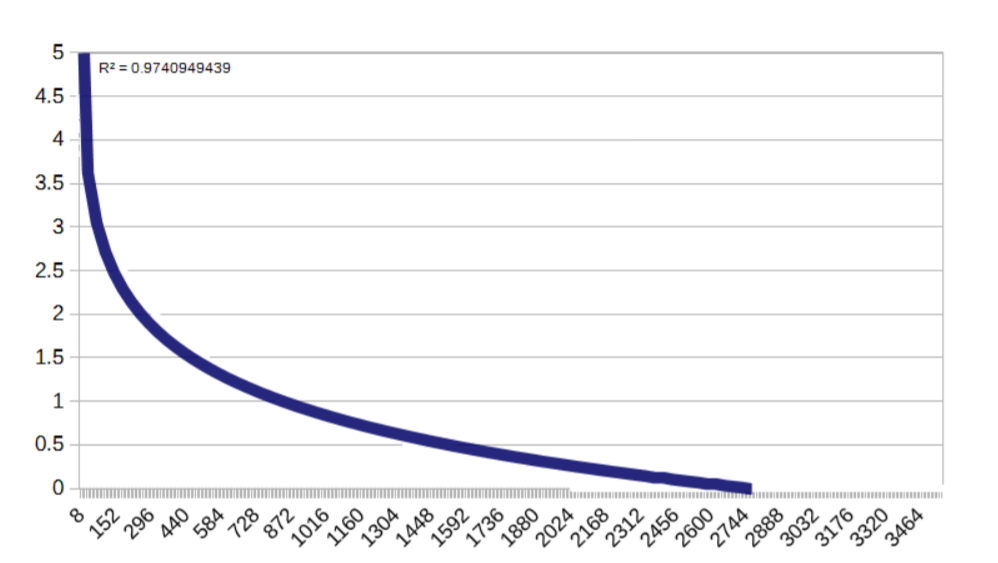
\includegraphics[width=4.5in]{placeholder.png} %testucd
% where an .eps filename suffix will be assumed under latex, 
% and a .pdf suffix will be assumed for pdflatex; or what has been declared
\DeclareGraphicsExtensions.
\caption{Exponential decay of contractions, relative to frequency.}
\label{fig:abb}
\end{figure}

%Figure 1: Exponential curve of contraction candidates
\VerbatimFootnotes

Contractions were predominantly non-standard English words. \hl{ The same truncated version of SCOWL}\index{Spell Checker Oriented Word Lists}, as described in Section \ref{section:prescription-solution} (totalling some 50,000 words), was used for reference. By using regular expressions to find characters  separated by repeating symbols,\footnote{\vspace{-24pt} \begin{verbatim}     i.e. (\w+)\s+(\w\w\w)\s+\d+\s}\end{verbatim}} and retrieving lexemes that were non English words, the frequency of all non-dictionary lexemes less than six characters in length were recorded. Contractions that appeared in different forms (e.g. a+e and A\&E) were counted together. As anticipated, contraction candidate frequencies followed an exponential distribution as seen in Figure \ref{fig:abb} (y axis scale is
log\textsubscript{10}). As expected also, the vast majority of unique lexemes collected were, in fact, unintentional spelling errors. These errors greatly contribute to the long tail of candidate frequencies visible in Figure \ref{fig:abb}.

While this underpinned the value that the identification of true positive contractions would have on the process of removing textual errors, it also indicated that frequency was a key feature of true positive contractions.


\subsection{Classification}

While we made efforts to look at potential semantic structures of lexemes which represented true positive contractions, in terms of both the occurrence of vowels and consonants, and potential phonetic structures which could be derived, no consistency between true positives could be determined using such a methodology. Unfortunately, using an N-gram-Over-Context model (NOC)\cite{kawamae2016n} similarly provided little better than random results in testing, as contextual features varied wildly for different types of contractions. Instead, features of candidate contractions were extracted based upon syntactic characteristics, with the value determined by frequency. As contraction frequency distribution was exponential, with a long tail of potential candidates, frequency values were consequently discretised into quartiles. Syntactic features were related to use of case (where the context was dissimilar), composition using symbols, and symbol suffixes. The absence of all the above characteristics was also derived as a feature. Originally, candidate length was also used as a feature, but this was later discarded due to it having a mildly negative impact on classification
accuracy.

250 candidates were randomly extracted for training purposes. These candidates were next classed as either true or false positives by domain experts. Taking a two-third training and one-third testing split, candidate contractions were examined by three separate classifiers.

\begin{table}[h]
\setlength{\tabcolsep}{0.5em}
\begin{center}
\renewcommand{\arraystretch}{1.5}
\begin{tabular}{|l|l|}
\hline
\textbf{Classifier}                    & \textbf{F1-score} \\ \hline
Decision Tree                 & 0.88     \\
Naive Bayes                   & 0.91     \\
Linear Support Vector Machine\index{Support Vector Machines} & 0.72     \\ \hline
\end{tabular}

\end{center}
\end{table}

As Naïve Bayes\index{Naïve Bayes} had performed well, and features were logically independent of one another, this classifier was chosen to identify true-positives within the corpus. 


\subsection{Repository Voting}

To the end of developing a system to inflate contractions to their full length forms, we approached a number of domain specific repositories with the aim of both achieving a comprehensive list of full length descriptions and the provision of disambiguation. The repositories used were the structured list of medical
abbreviations on Wikipedia, the official list of abbreviations produced by the Irish Health Service Executive, and Acromine\index{Acromine}'s RESTful API populated from Medline\index{Medline} \cite{okazaki2006building}. Both Wikipedia and Acromine\index{Acromine} provide disambiguated results, while both the HSE and Wikipedia consist of manually written entries.
In the event of a particular contraction being provided multiple definitions by one of the repositories, these definitions would be compared with any definitions that may be provided by the other repositories. If a
non-disambiguated match could be made, this definition would be chosen; otherwise a majority vote between
repositories would be performed, with the most frequent entry within Acromine\index{Acromine} taken as the definition from
that repository. In the event of a disagreement for a particular definition between any two repositories, a similar voting procedure would
take place. If a consensus could not be reached between the repositories, no definition was chosen. 

In order to achieve this mechanic some cleaning of all repository entries had to be performed (Wikipedia had any text occurring within a final set of parentheses deleted, as these were typically notes describing etymology or term usage). Exact matches were not required in the voting mechanic, and in the event of string similarity the longer candidate was chosen to as the definition for the contraction.

After entries with conflicting definitions in more than two of the repositories were deleted, the following list of definitions was generated. The process described as “Uncontested” refers to the scenarios where the definitions present have no conflicting definitions within other repositories.

\subsection{Word Embeddings}
\label{section:word_embeddings}


 Word Embeddings are low dimensional distributed representations
of words in a real-valued vector space. These are richer data than available in atomic representations of lexemes (i.e one-hot vectors). Due to their capacity to exhibit semantic similarity, the use of word embeddings as a form of representation have become increasingly popular in the area of NLP\index{Natural Language Processing} \cite{goldberg2017neural}. We created word embeddings with the Gensim implementation \cite{rehurek_lrec} of Word2Vec\index{Word2Vec}, using the Skip-Gram model \cite{guthrie2006closer}. This was trained using a length of 100, and windows of 5 (i.e. the maximum distance between the current and predicted word within a sentence). This training was done with a partially preprocessed version of the corpus itself being used as the training data. This preprocessing converted all words to lowercase and removed all non alphabetic characters, after tokenisation. Sentence disambiguation was also employed on this dataset. 

Although this  methodology is non-typical in the training of the Word2Vec\index{Word2Vec} unsupervised neural network, with most researchers using a pretrained version \cite{feng2019deep,khatua2019tale,orkphol2019word}, the rationale for using the corpus for training was due to the high frequency of domain specific terms and local jargon that would appear infrequently in corpora populated from sources such as news outlets. In particular, contractions and acronyms may exactly resemble common words habitually present in most corpora, but have distinct meaning within the context of the medical institution in question (e.g. ``sob" a word which typically refers to the process of crying, specifically means ``shortness of breath" in the dataset in question). Our data of word embeddings also maintained the inherent structure present in patient medical notes, as this would likely prove beneficial for neural network architectures which would have the capacity to recognise such structural patterns.    



\begin{table}[]
\ra{1.5}
\setlength{\tabcolsep}{0.7em}
\caption{Definition list}
\label{table:acc_source}
\begin{center}
\begin{tabular}{|lll|}
\hline
\textbf{Source}                          & \textbf{Process}                            & \textbf{Results} \\ \hline
\multicolumn{1}{|l|}{Wikipedia} & \multicolumn{1}{l|}{Uncontested} & 1339    \\
\multicolumn{1}{|l|}{}          & \multicolumn{1}{l|}{+ Acromine\index{Acromine}}    & 31      \\
\multicolumn{1}{|l|}{}          & \multicolumn{1}{l|}{+ HSE}         & 325     \\ \hline
\multicolumn{1}{|l|}{HSE}       & \multicolumn{1}{l|}{Uncontested} & 722     \\
\multicolumn{1}{|l|}{}          & \multicolumn{1}{l|}{+ Acromine\index{Acromine}}    & 42      \\ \hline
\multicolumn{1}{|l|}{Acromine\index{Acromine}}  & \multicolumn{1}{l|}{Uncontested} & 4020    \\ \hline
\textbf{Total}                           &                                    & \multicolumn{1}{|l|}{ 6484}    \\ \hline
\end{tabular}
\end{center}
\end{table}



A distinction arose between acronyms and abbreviations when finding full length forms. Abbreviations tend to be more colloquial and are more susceptible to neologisms. The exhaustive nature of the long version deduction, combined with the specificity of the resources used, initially produced flawed results with some common abbreviations. For instance "ok" was correctly classified as a contraction, but resolved to Opposum Kidney instead of "okay" due to a high occurrence of this acronym within Medline\index{Medline}. Similarly, the abbreviation "pt" was interpreted as the acronym for “prothrombin time” rather than the intended meaning of "patient".

Word2Vec\index{Word2Vec} was accordingly used to find semantically similar lexemes to the contractions classified as true-positives. In the case that syntactic similarity between a candidate and its vectors was identified, that vector was chosen as the
long form of the candidate. These vectors included both English words and other contractions.
Many of the long forms derived from word embeddings represented forms which were not necessarily
correct, but were closer to their correct form than initially presented. For instance the abbreviations symps
and sympt were expanded to the form “sympotms”, while pres was expanded to “prescreption”. These
misspellings represent very small edit distances from the correctly identified long form, making their
correction in post-processing a relatively trivial task. This process also included the clustering of different
contractions, such as phx and pmhx, which both represent “past medical history”. Unfortunately “pmhx” was
itself too morphologically dissimilar from its long form “history” to successfully provide a derivation
(“history” had a cosin distance of 0.54 from pmhx). 32.43\% of contractions which were substituted by a
semantic neighbour were changed to a better lexicological form in this manner.

Of other semantic substitutions, 37.29\% represented an exact match with their long form (or synonymous
lexeme), while 19.45\% were expanded to incorrect long forms. Incorrect long form substitution included
“lrti” to “laryngitis”, where “lrti” is an acronym meaning “lower respiratory tract infection” and laryngitis is
a specific respiratory tract infection (which is often in the upper respiratory tract). Similarly “opd”, an
acronym meaning “out-patient department” was incorrectly associated with “orthopaedic”. A further 10.27\%
of substitutions provided no substantial improvement (such as the clustering of om and som, which relate to
slightly different conditions (otitis media versus serous otitis media respectively)). Also it must be noted that
typographical errors could be incorrectly associated with a long form in this process, particularly in the case
of shorter abbreviations. For instance, “f” was associated with the abbreviation fallw (which itself stands for
“follow”). However in almost 7\% of cases, “f” is actually an incorrectly written version of the word “of”.



\subsection{Results}

Testing in relation to the contractions was performed in relation to 150 randomly selected cases, totalling
some 7251 words \hl{(which in turn contained 1239 contractions)}. Manual analysis of each of these cases was performed, providing the results in Table \ref{table:acc_inflation} below.

From Table \ref{table:acc_repository}; simple lookup of repositories for long forms of contractions accounted for a large percentage of long forms obtained, or 38.18\% of the total, but repository voting added an effective way to extend the number of long forms that could be obtained from repositories (accounting for some 12.61\% of total long form sources). Using repositories as a source for long forms was more accurate than using word embeddings (Table \ref{table:acc_inflation}). 

The repositories used, despite all relating to the medical domain, were significantly divergent in the manner in which they had been composed. While the HSE data was written by a small number of health professionals, the Wikipedia data was open to modification by any member of the public (and had hundreds of editors). In counterpoint the Acromine data was automatically generated. The difference means employed to compose these lists is reflected in the volume of long form candidates generated by the respective repositories (Table \ref{table:acc_source}).\hl{ It is self-evident that the larger volume of editors for Wikipedia resulted in a significantly larger number of definitions than that available in the HSE list. Similarly, the automated nature of Acromine accordingly generated a very large number of definitions which were not present in the other repositories.} 

In testing, the results of which are visible in Table \ref{table:acc_inflation}, long forms were found for 97.4\% of candidates classified as contractions, of which 82.76\% were correct. The program achieved a recall of 0.90. The program, from start to finish (from contraction detection to long form generation), achieved an f-score of 0.86.

% Please add the following required packages to your document preamble:
% \usepackage{booktabs}
\begin{table}[h]
\ra{1.3}
\setlength{\tabcolsep}{0.6em}
\caption{Abbreviations and Acronyms Identification within Test Data.}
\label{table:acc_inflation}
\centering
\begin{tabular}{@{}l|l|l|l@{}}
\toprule
Type         & Description                & Number & Precision \\ \midrule

Short        & \textbf{No inflation}      & 31     &           \\
Long         & \textbf{Inflation}         & 1120   &           \\
             & \hspace{3mm}\textbf{from repositories} &\hspace{3mm}557    & 0.87      \\
             &\hspace{3mm}\textbf{from embeddings}   &\hspace{3mm}563    & 0.78      \\
Undiscovered &                            & 88     &           \\
Total        &                            & 1239   &           \\
\bottomrule
\end{tabular}
\end{table}

Results over the entire corpus can be seen below in Table \ref{table:acc_repository}

% Please add the following required packages to your document preamble:
% \usepackage{booktabs}
\begin{table}[h]
\ra{1.3}
\setlength{\tabcolsep}{0.6em}
\caption{Long form sources.}
\label{table:acc_repository}
\centering
\begin{tabular}{@{}l|l|c@{}}
\toprule
\textbf{Expansion source}  & \textbf{Total}  & \textbf{Percentage of whole} \\ \midrule
Repository        & 727056 & 38.18               \\
Repository voting & 240196 & 12.61               \\
Word embedding    & 936848 & 49.20               \\
No long form      & 30944  & 1.6                 \\ \bottomrule
\end{tabular}
\end{table}

\subsection{Discussion}

\hl{Although in an ideal world, a foolproof approach to the problem established in this section would appear to be the generation of a hand curated list of contractions with their long form counterparts, written by a domain expert working with the particular dataset in question, in reality such an approach would likely to be both costly and inaccurate. A scalable approach is necessary to treat morphological disparities between different users, adjustments in use over time, and neologisms.}      

This section details a suitable means to address poor quality medical text where the use of abbreviations and acronyms may be habitual, but may have poor identifying features. Moreover, where definitions for contractions are not provided in the text under examination, this chapter outlines a successful approach to automatically choose the most likely suitable long form. The ability to provide the expansion of abbreviations promises greater potential interoperability between different systems, or comparisons between corpora. While identifying true positive contractions can be useful to prevent accidental deletion in potential automated spelling correction processes, the primary value lies in consolidation of features to more generic forms.

While the classifier described above accurately detects contractions, it does not distinguish between abbreviations and acronyms. This can have negative consequences when attempting to correctly attribute long forms to their respective contractions. While there is unlikely to be any method that will be able to perfectly distinguish the two, morphological characteristics can potentially be used to gain a confidence measure in deciding between these respective entities. Similarly, Soundex could potentially be used to obtain more accurate association of abbreviations to their long forms, though this again is unlikely to provide a catchall solution. A more significant consideration is that while the methodology outlined in this research takes a context sensitive approach when considering contraction candidates and their potential meaning as a whole, it does not consider context in relation to individual contractions in the task of textual substitution. Where spelling errors and overloaded use of contractions can occasionally occur, providing a means to exclude false positives could improve final results.

\section{Treatment of symbols}

One final important consideration in relation to the FTN was the presence of symbols that did not fit into any of the usage cases outlined above. While NLP\index{Natural Language Processing} research may discard symbols as part of standard cleaning and tokenisation operations, casual observation of the Caredoc\index{Caredoc} data showed extended use of symbols in semantically important roles. For instance, exclamation points may be used to indicate important findings, two addition symbols may indicate escalation, and details may be segmented using ellipses.  

The treatment of these symbols was fairly straightforward. Using regular expressions all repeating symbols were replaced 
$\forall \textit{ |s| } > 1 : s \longrightarrow T, \textit{s} \in S $. Where \textit{S} is the set of non-alphanumeric characters and T is a unique token. 

\hl{An example of this symbol replacement, and also the contraction identification and replacement described in Section} \ref{section:abbreviations&acronyms}, is visible in Figure \ref{fig:word-replacement}.  In the final version of preprocessed text, tokens indicating that a token was identified as a  contraction was added to the text (prepending the contraction or the long substitute). This token would, if applicable, also indicate the manner in which the long version of contractions was derived (be it from a repository, repository voting, or from word embeddings). This same approach was adopted in relation the medications identified in Section \ref{section:medication-reconciliation}.    

Sentence disambiguation was a simple process once contractions had been identified. Periods that were part of numbers, abbreviations, acronyms, and ellipses were removed, and all other usage of periods was considered to relate to sentence terminators. The same applied to the use of newlines. Because capitalisation was so inconsistent, and as mentioned earlier, typical English grammar was often omitted, a more sophisticated solution seemed neither feasible nor profitable in this context.  




\begin{figure}[htbp]
   \begin{center}

 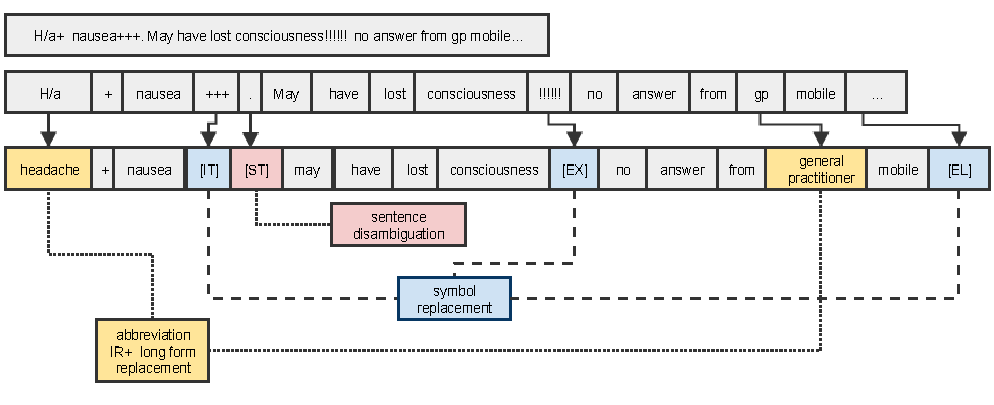
\includegraphics[width=1.0\textwidth]{Figs/scheme-word-replacement.pdf} 

 \caption{Sample FTN text featuring basic symbol replacement}
 \label{fig:word-replacement}
  \end{center}
\end{figure}

\begin{comment}
!!!!!!!!!!!!!!!!!!!!!!!
Similar to twitter 
!!!!!!!!!!!!!!!!!!!!!!!!!!!!!!!!!!!!!!
\end{comment}

\section{Impact on corpus}
\label{section:preproccesing-impact-on-corpus}

So far in this chapter the treatment of the various aspects of the medicinal text has been isolated from the ultimate impact on the dataset as a whole. While the information retrieval, clustering, and transformation methodologies developed to this end have value in themselves, their main relevance within the scope of this thesis is their impact on the ultimate performance of the frequent user classifier.  

This section will provide details on the changes that this preprocessing has affected in relation to the FTN as a whole. While dimensionality reduction was an aim of the preprocessing described in this chapter, this did not mean that data reduction was a goal.

The preprocessing described in this chapter was an iterative process, and the eventual output was guided by initial results provided by ANN architecture testing. As this testing progressed, and it became clearer that a model that could understand patterns relating to the sequence of input (or at least the immediate context of input) was likely to be more successful in classification, the choice was made to include information relating to the preprocessing tasks into the text itself.

By reducing the number of symbol patterns it was hoped that a machine could more easily interpret the intended meaning of such patterns. The same was true for numbers. Instead of having strings of numbers interpreted as unique lexemes, all numbers (integers, real numbers, etc.) would be discretised to a general token representing numerical strings. This is because even machine learning algorithms that could understand textual context would have to see each of these numbers multiple times in the same sort of environments to work out that were, in fact, numbers. Because of the large volume of unique numbers in the dataset, there would be many instances where the machine learning algorithm would inevitably fail to make this connection. While discretising numbers in this fashion was going to lose the scalar data from the FTN, this information was unlikely to ever be useful. While a context like "patient has temperature of 42 C" provides much more value, from a medicinal point of view, than "patient has a temperature of numtoken celsius", there are a vast number of different contexts within which numerical values arise; and these contexts were often not recorded in a particularly consistent manner. For instance the above example could be written: "pt temp 107.6.". 

Relating back to the free-text\index{free-text} data described in Section \ref{section:free-text-description}, the volume of additional data generated by the processes described in this chapter can be seen in Table \ref{table:corpus-preprocessed}, with the change presented in brackets. The change in unpreprocessed text \textbf{P} and preprocessed text \textbf{P'} also shows a significant drop in the number of unique words present in the text. Note that a very large number of the unique lexemes remaining in the corpus are single instance spelling errors. Although it is the contention of this thesis that the steps detailed in this chapter would no doubt support any subsequent attempts to address these spelling errors (as important terms in the form of contractions would be less subject to type two errors in any hypothetical automated spell correction program) the actual development and deployment of such an effort is outside the scope of the preprocessing steps being considered in this chapter.    


\newcommand{\forceindent}{\leavevmode{\parindent=2em\indent}}






\begin{table}[h]
   \ra{1.3}
\caption{Free-text data in preprocessed corpus.}
\label{table:corpus-preprocessed}
\begin{center}
\begin{tabular}{|l|c|c|c|}
\hline
\textbf{attribute}     & \textbf{entries} & $\mathbf{\bar{c}}$ & $\mathbf{\bar{w}}$   \\
\hline
olc\_history   & 15226  & 212.86 (+30.14) & 34.01 (+17.43) \\

olc\_examination & 11326  & 148.13 (+33.13) & 22.65 (+15.41) \\

olc\_diagnosis & 120433  & 36.04 (+10.58)  & 5.13 (+3.47)  \\

olc\_treatment    & 123517  & 122.08 (+47.22)  & 17.11 (+11.5) \\

teleguides & 58906 & 315.17 (+43.89)  & 49.95 (+11) \\
\hline
\end{tabular}
\end{center}
\label{table:free-text}
\end{table}

% Please add the following required packages to your document preamble:
% \usepackage{booktabs}


\begin{table}[ht]
\forceindent
\begin{tabular}{|l|cc|}
\hline
                  & \multicolumn{1}{c}{\textbf{P}} & \multicolumn{1}{c|}{\textbf{P'}} \\  
Unique words      & 131841                         & 114507                           \\
Lexical diversity & 0.072                          & 0.069                            \\ \hline
\end{tabular}

\end{table}


\begin{comment}

\begin{table}[ht]
\begin{tabular}{|r|cc|}
\hline
               & \multicolumn{1}{l}{\textbf{Unique words}} & \multicolumn{1}{l|}{\textbf{Lexical diversity}} \\  
Unpreprocessed & 131841                                      & 0.072                                           \\
Preprocessed   & 114507                                      & 0.069                                           \\ \hline
\end{tabular}
\end{table}


\end{comment}






\section{Summary}


This chapter detailed some of the major steps taken in preprocessing the FTN contained within the corpus. This research is agnostic in relation to potentially encouraging users to improve their methods of recording information in free-text fields. Instead, scalable machine learning approaches have been presented that can automatically process domain specific terms. While accepting that the data contained within FTN were noisy and highly heterogeneous, this chapter attempted to develop means of processing the text that would reduce this noise and heterogeneity while respecting the integrity of the information contained within case notes. Attempting to fix errors and reduce noise, without inadvertently destroying valuable information, is a challenging process; as is evidenced by the methodologies discussed in this chapter. Notwithstanding their impact on the classification processes described in Chapter \ref{chpt:predictive-modelling}, these cleaning and clustering methodologies also have relevance in other medical contexts.   
